\section{Method and results}
\protect\label{section:results}

The following approach was taken to analyse the data.

Please note that much of this initial work was done with available data up to
the end of October 2018. There has been later date available in July 2019, but
the images and analysis below were propared before then.

\subsection{Intensity comparison}
\protect\label{section:intcomp}

As a first attempt to study the data, I took the ADU count, specifically the net after applying the flat and bias files
of the target in all the images in which it was available. The target was found in all of the images, apart from in some of the
\textbf{g}, \textbf{i} and \textbf{r} visible light filters, as shown in Table \ref{table:occtb} below.

Plotting light curves of the intensities obtained in this way yields Fig. \ref{fig:allall}.
Binning the intensities together into a single day gave
Fig. \ref{fig:allbin}, the error bars indicate the spread over a single day. I plotted
periodograms, as shown in Fig. \ref{fig:pgrams}. Despite the crudeness of the data, it is noticeable that there are
peaks close to the rotation periods of the order of 150 days referred to in \citet{suarezmascareno15} and \citet{toledopadron18}.

\begin{figure}[!htbp]
\begin{center}
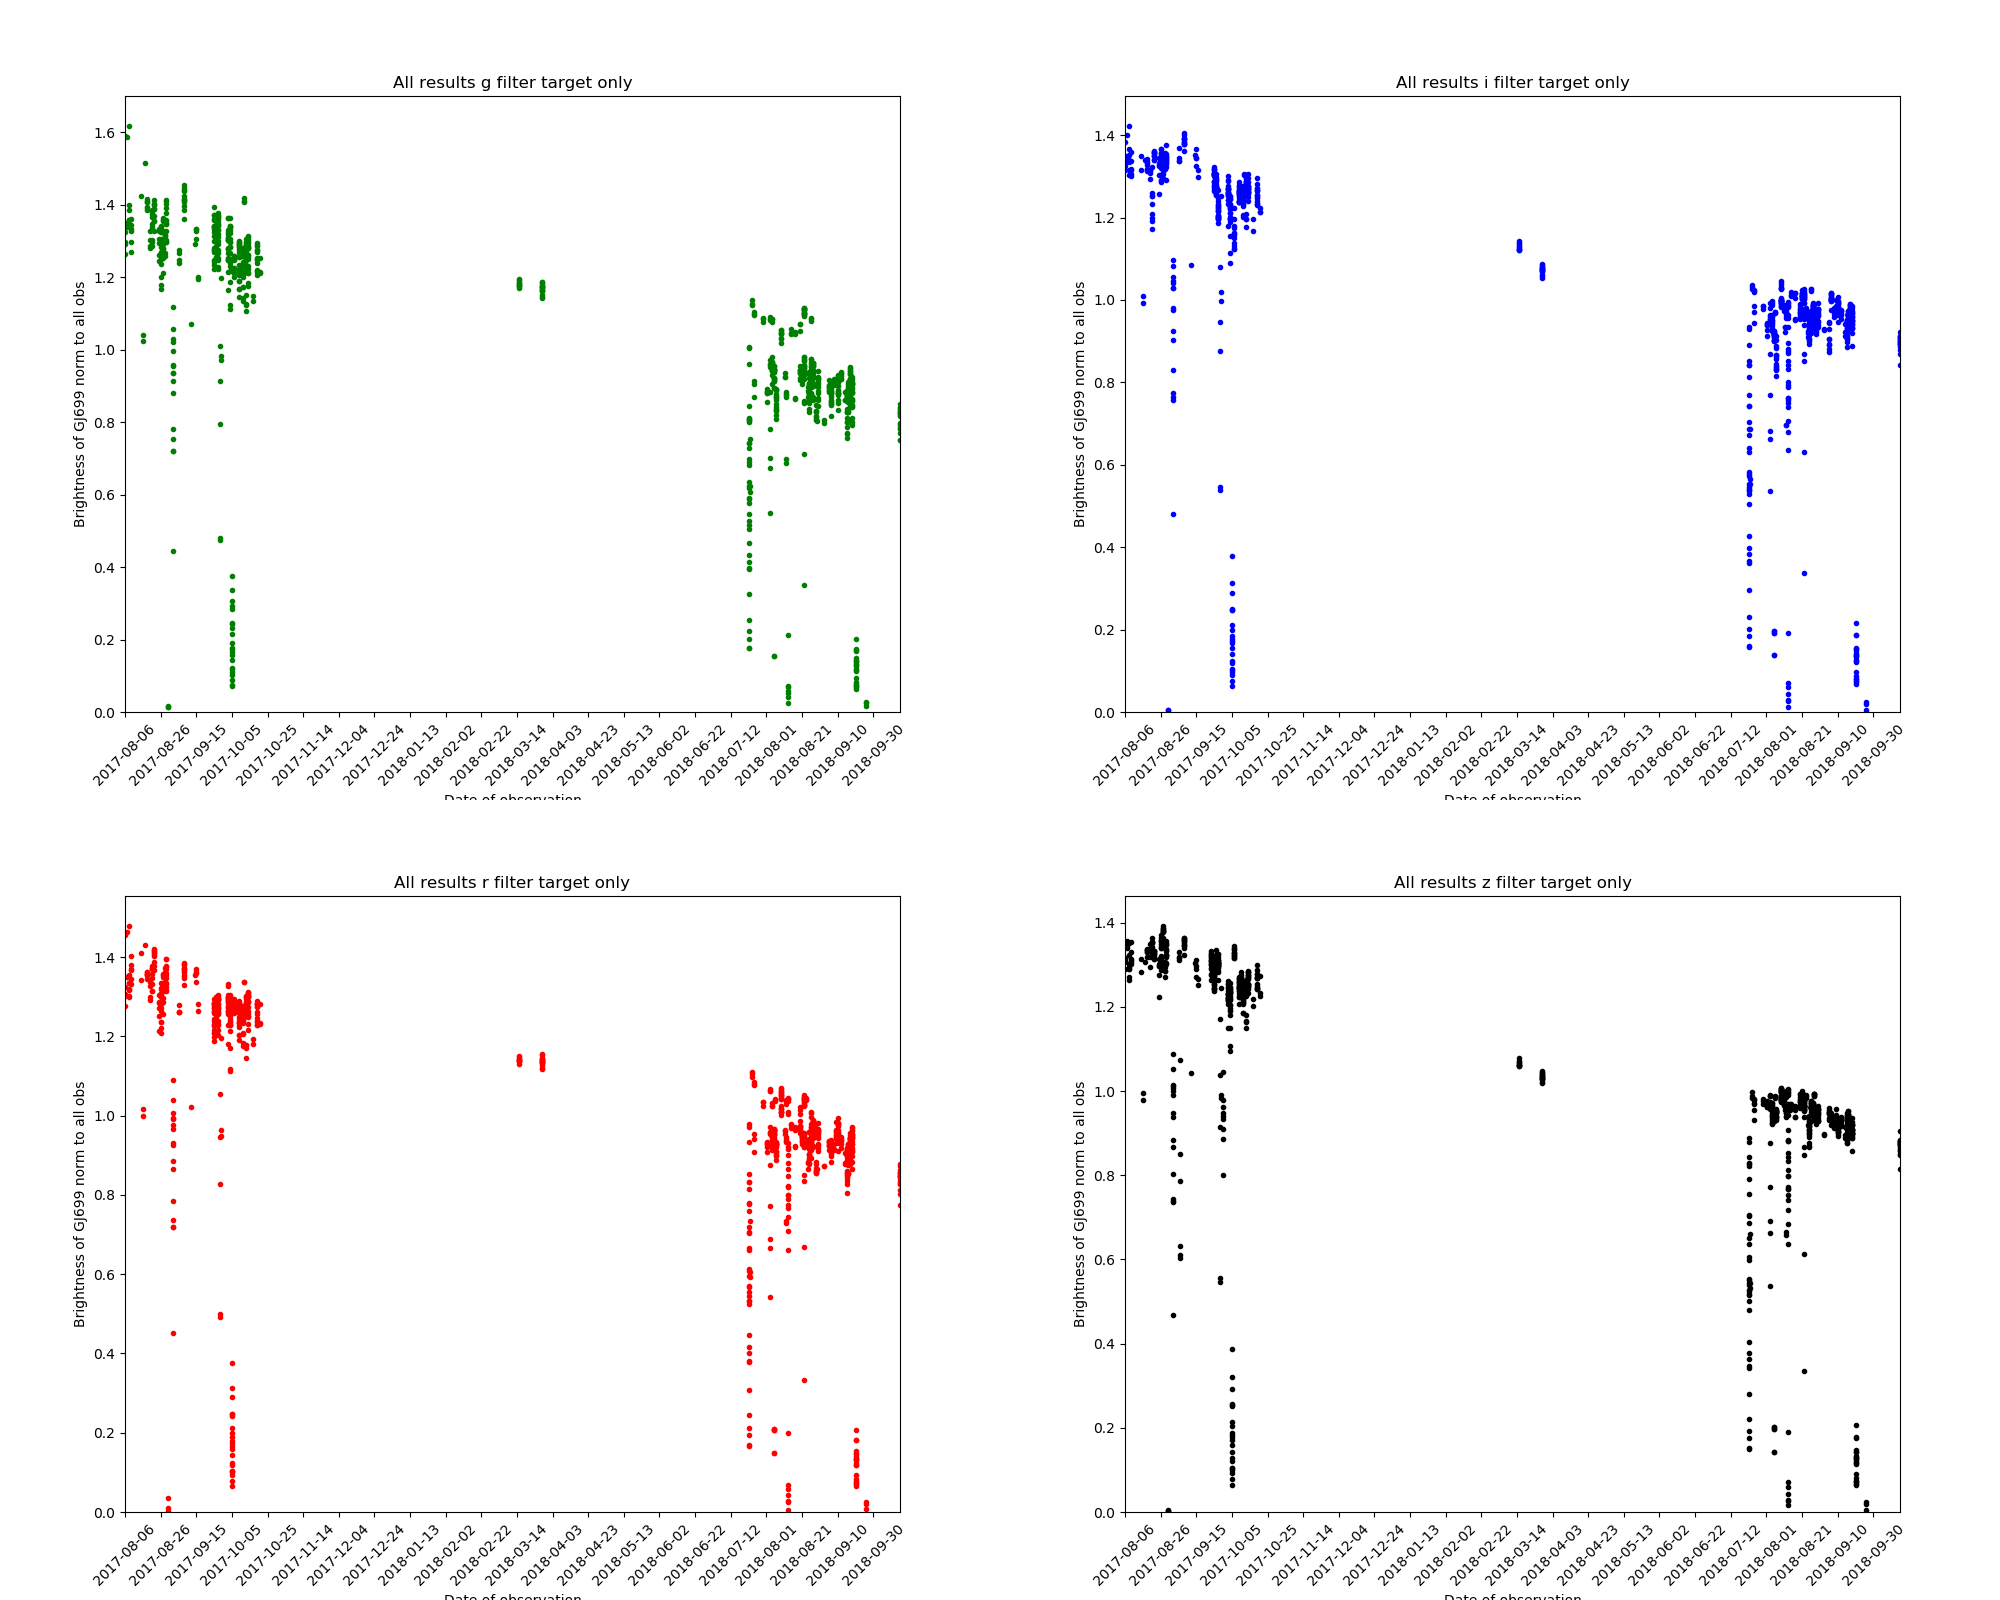
\includegraphics[scale=0.25]{images/allall.png} \\
\end{center}   
\caption{This shows the flux for the target, \bstar, for each of the four visible light filters. This takes the total
  ADU count only}
  \protect\label{fig:allall}
\end{figure}

\begin{figure}[!htbp]
\begin{center}
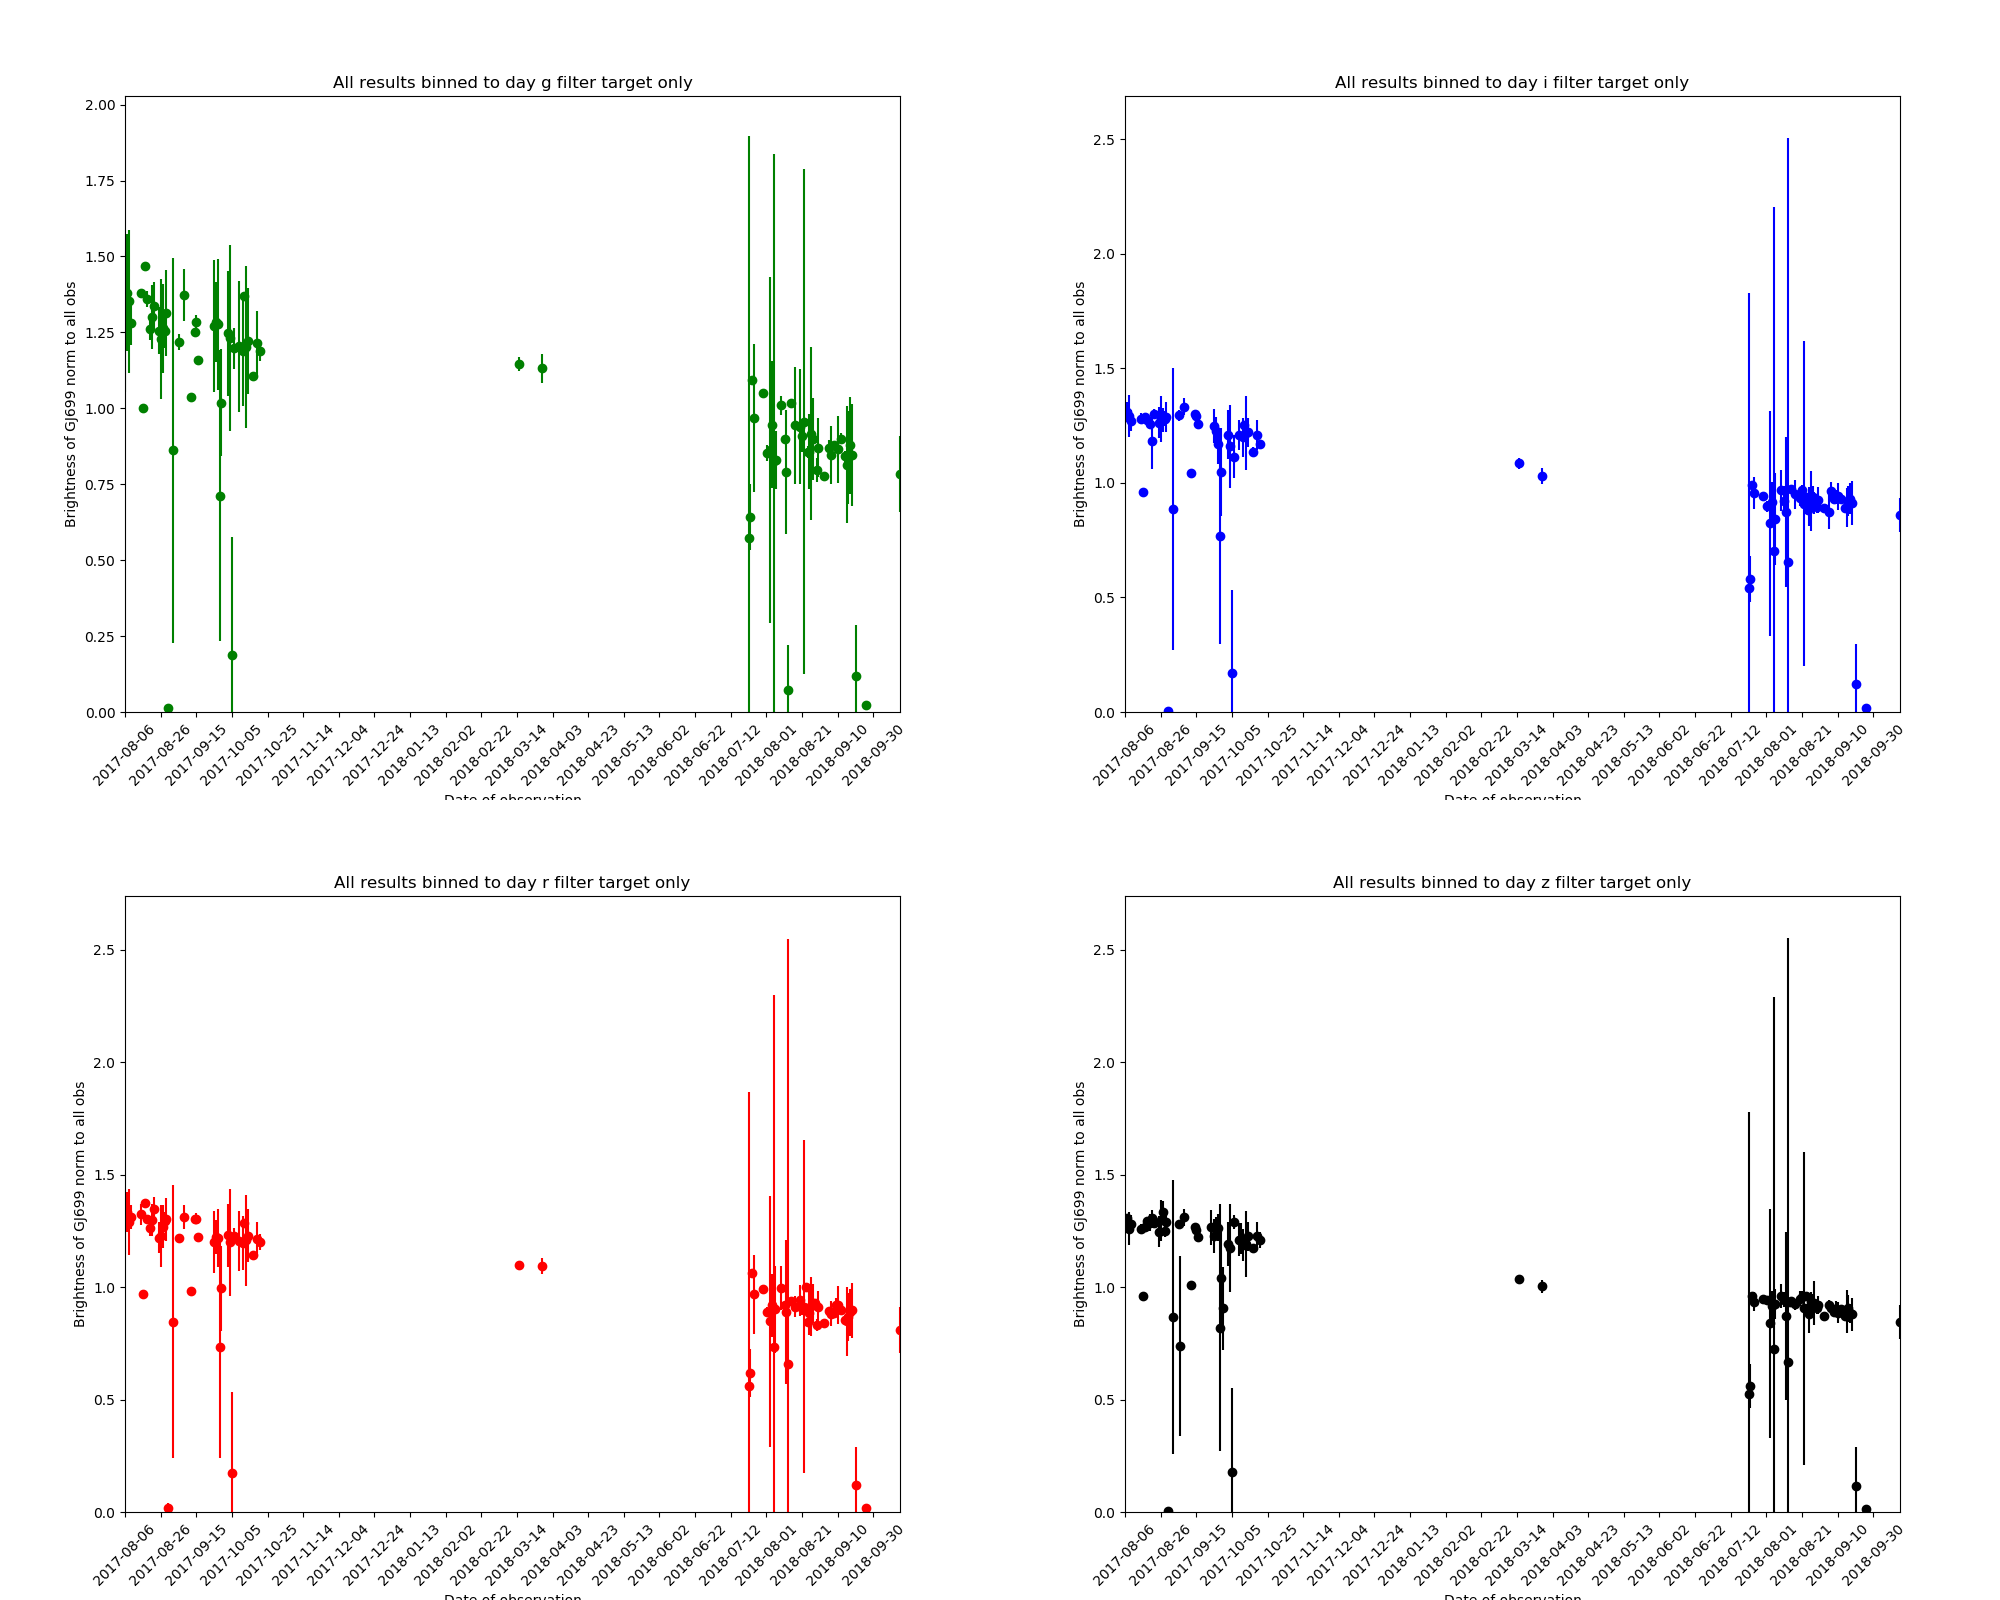
\includegraphics[scale=0.25]{images/allbin.png} \\
\end{center}   
\caption{This shows the flux for the target, \bstar, for each of the four visible light filters and binned to a single day. Error bars are show to indicate the spread of intensities over a single day.}
  \protect\label{fig:allbin}
\end{figure}

\begin{figure}[!htbp]
\begin{center}
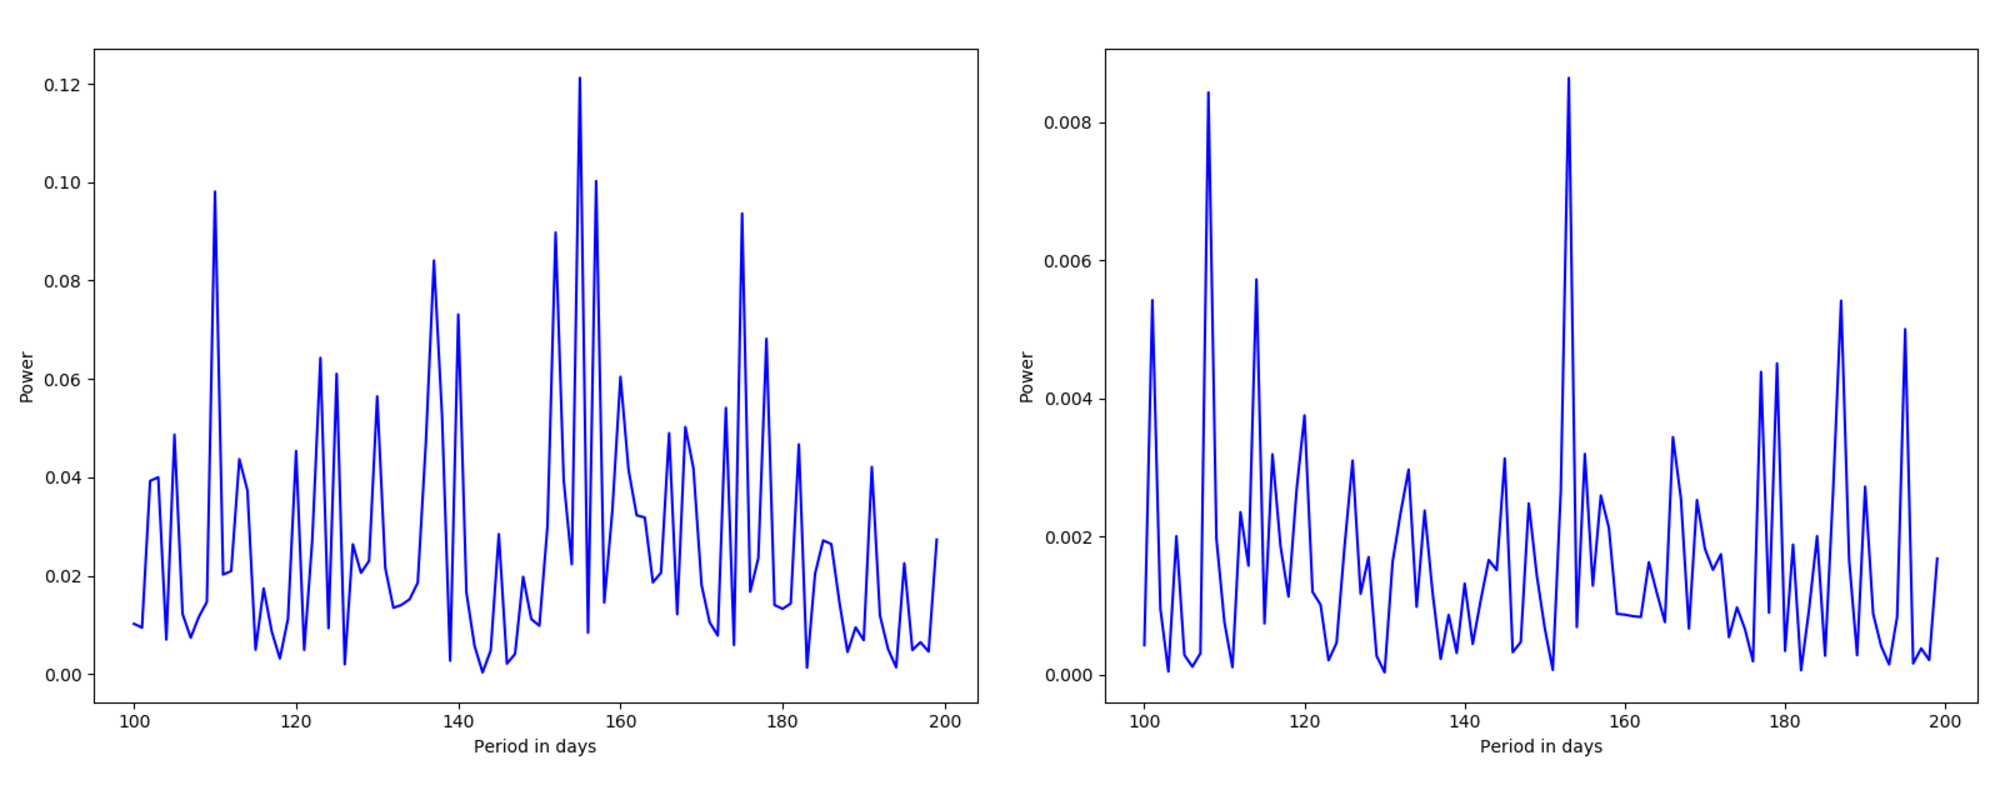
\includegraphics[scale=0.25]{images/pgrambunb.png} \\
\end{center}   
\caption{This displays periodograms derived from the binned (Fig. \ref{fig:allbin}) and unbinned
  (Fig. \ref{fig:allall}) light curves for the \textbf{r} filter.}
  \protect\label{fig:pgrams}
\end{figure}

It is accepted that this initial treatment is crude. Serious work needs to be done on correction for air mass,
which for a few observations, where they are spread over a period of several hours,
can be quite large, and to more accurately discard as unacceptable images with large or very variable sky levels.
There are some currently inexplicable variations, for
example the to images in Fig. \ref{fig:tyeg} give radically different ADU counts despite being taken two minutes apart
with same exposure time and other parameters.

\begin{figure}[!htbp]
\begin{center}
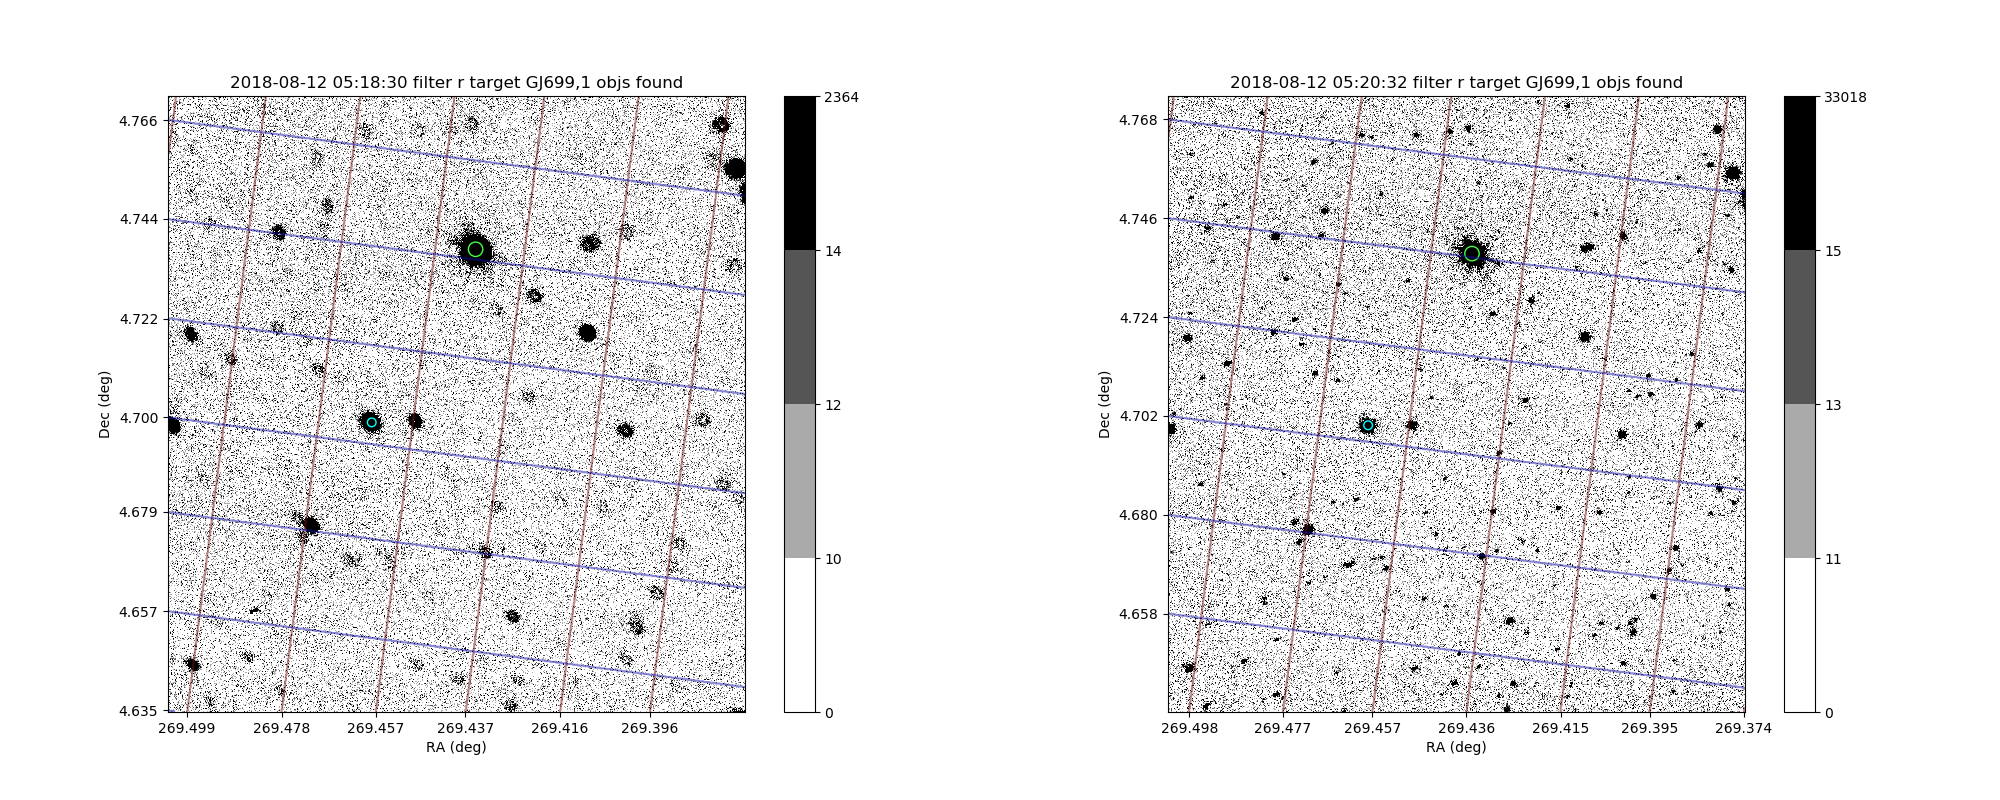
\includegraphics[scale=0.25]{images/tyeg.png}
\end{center}   
\caption{These images show an example of where 2 images taken 2 minutes apart with the same exposure time gave different flux values.}
  \protect\label{fig:tyeg}
\end{figure}

\subsection{Reference Stars}
\protect\label{section:refstars}

Rather than relying on the ``raw'' flux from the target star itself, I made an approach based on identified reference
stars found in a significant number of images. Ideally these should be as many as possible to ``smooth'' out errors and
variations on the reference star. By taking the ratio of the target star ADU count to the sum of the reference star
ADUs, then we can hope to achieve results for intensity with the factors such air mass corrections factored out, This
approach was taken in \citet{berry11} and would seem to involve least work, provided sufficient reference stars are
consistently found.

The algoritm used to find objects was first to locate the target (there was
usually a certain amount of error in the coordinates of the images) and then
find prefeviously-known reference objects. The criterion for finding objects was to look for groups of pixels within a
given scan aperture whose mean count was a given number of standard deviations
(intially 3) from that of the sky level. If the result appeared to be one of
the objects known already, the given reference object was deemed to have been
found.

To initialise the database of objects, I used Simbad, 2MASS and SDSS to find objects in the vicinity of \bstar, obtaining the following stars as shown in Table
\ref{table:reftimesfound}. Of the stars there, the types are unavailable apart from the most-frequently occurring one of
TYC425-262-1, which is an A3V star (this is also reported as the most frequently found reference star in \citet{berry11}).

\begin{table}[!htbp]
\begin{center}
\begin{tabular}{llr} \hline
Number & Object & Times found \\\hline
1 & TYC425-262-1 & 5,277 \\
2 & SDSS1237671695527248969 & 3,408 \\
3 & 2MASSJ17574653+0447466 & 3,297 \\
4 & SDSS1237668573088841773 & 840 \\
5 & TYC425-223-1 & 369 \\
6 & SDSS1237671695527249415 & 15 \\
\hline
\end{tabular}
\end{center}
\caption{This lists the identified reference objects near to {\bstar} and the number of times found in the available
  data. Note that this data relates to images up to the end of October 2018.}
\protect\label{table:reftimesfound}
\end{table}

I decided to consider only the first 3 reference objects, which are labelled 1, 2 and 3 for convenience in the
remainder of this report, as the appearances of the others were too infrequent to render them worthwhile.

\subsection{Classification of results}
\protect\label{section:classresults}

The images presented challenges in various respects. The visible light images are all at different orientations and with
the target in different places in the image, so not all the reference stars appear in all of the images. In some cases
the reference stars are just not bright enough to rise sufficiently above the sky level.

\begin{table}[!htbp]
\begin{center}
\begin{tabular}{lrrrr}
&Filter g&Filter i&Filter r&Filter z\\\hline
Target not found&167&80&105&0\\
No ref objs found & 84 & 1,003 & 53 & 1,085 \\\hline
Obj 1 (with or without others) & 834 & 0 & 925 & 0 \\
Obj 2 (with or without others) & 561 & 1 & 574 & 0 \\
Obj 3 (with or without others& 526 & 0 & 573 & 0 \\
Obj 1 only & 43 & 0 & 100 & 0 \\
Obj 2 only & 0 & 1 & 1 & 0 \\
Obj 3 only & 0 & 0 & 0 & 0 \\
Objs 1 and 2 (with or without 3) & 561 & 0 & 573 & 0 \\
Objs 1 and 3 (with or without 2) & 526 & 0 & 573 & 0 \\
Objs 2 and 3 (with or without 1) & 296 & 0 & 321 & 0 \\
Objs 1 and 2 only & 265 & 0 & 252 & 0 \\
Objs 1 and 3 only & 230 & 0 & 252 & 0 \\
Objs 2 and 3 only & 0 & 0 & 0 & 0 \\
Objs 1,2 and 3 & 296 & 0 & 321 & 0 \\
\hline
\end{tabular}
\end{center}
\caption{This table shows the occurrences of the 3 main reference objects in each of the observations with or without
  the others. The infrared images were omitted as no reference objects were found in any of them. Note however the lack
  of occurrences of reference objects in the \textbf{i} and \textbf{z} filter images.}
\protect\label{table:occtb}
\end{table}

\subsection{Results from reference object comparisons}
\protect\label{section:refobjres}

Repeating the light curve plots from Section \ref{section:intcomp}, this time as the ratio of the ADU count of the
target to the sum of the first three reference objects, Fig.  \ref{fig:allref123} and Fig. \ref{fig:allref123bin} show
the light curves for the \textbf{r} and \textbf{g} filters. Also shown in Fig. \ref{fig:ls123both} are periodograms
derived from these light curves. Also shown in Fig \ref{fig:allref1}, Fig. \ref{fig:allref1bin} and Fig. \ref{fig:ls1both}
are the corresponding results taking into account only the brightest of the reference objects, TYC425-262-1.

\begin{figure}[!htbp]
\begin{center}
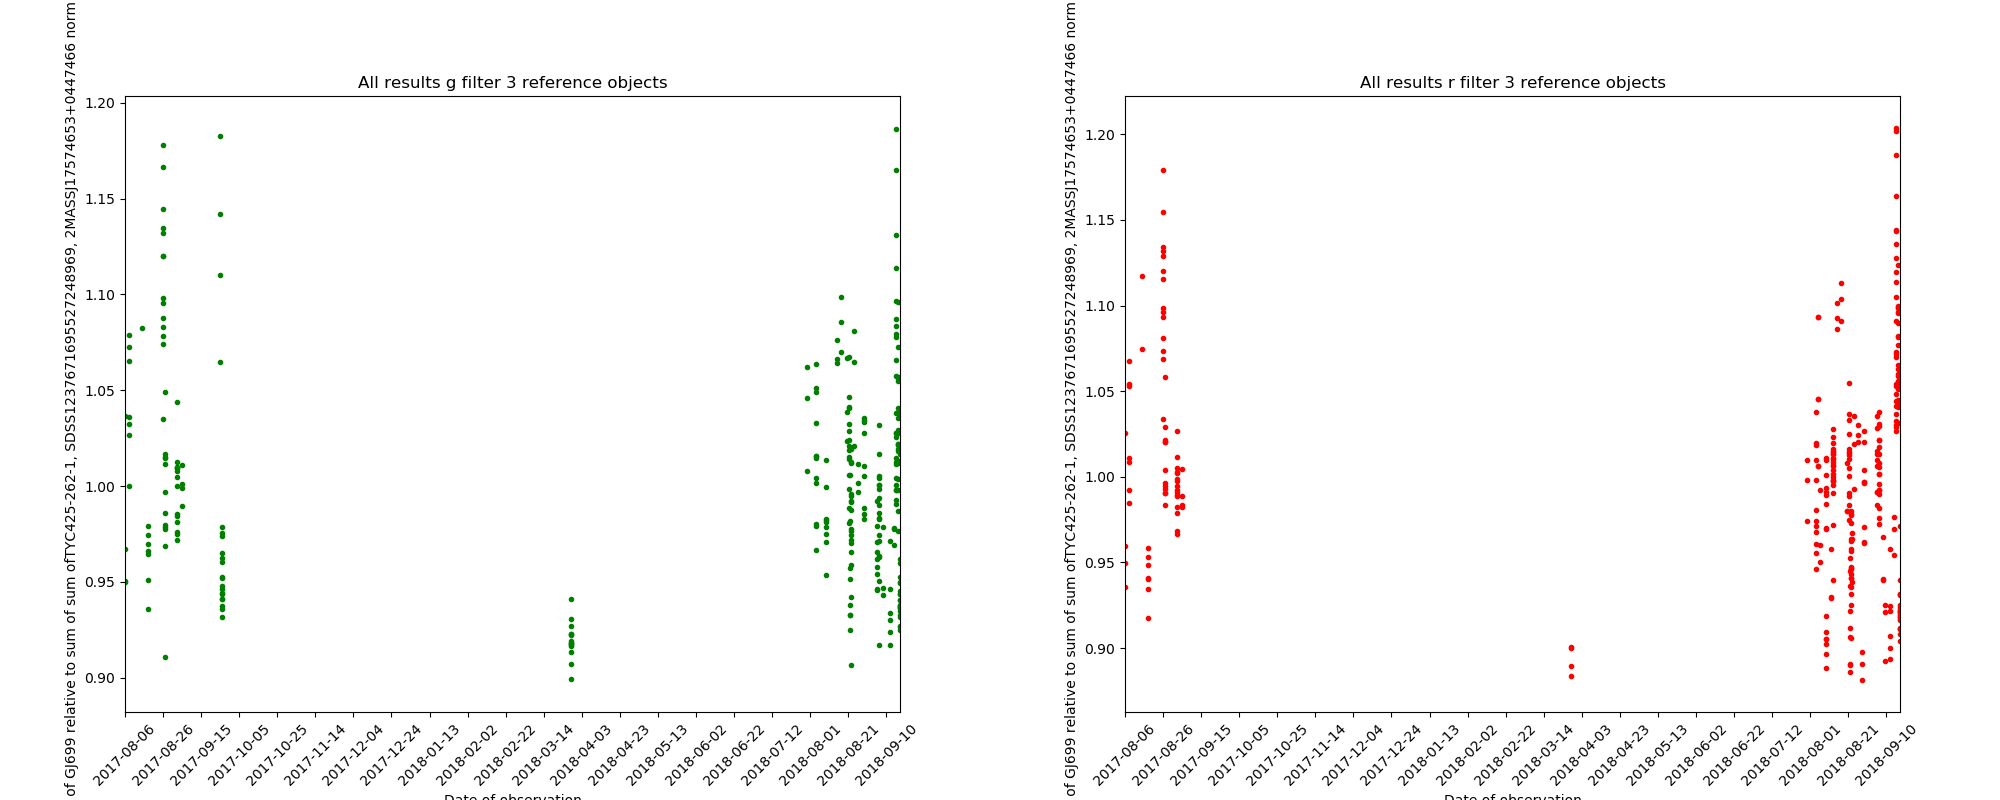
\includegraphics[scale=0.25]{images/allref123.png}
\end{center}   
\caption{This shows the ratio of the flux for the target, \bstar, to the 3 main reference objects for the \textbf{g} and
\textbf{r} filters, plotted as green and red respectively.}
  \protect\label{fig:allref123}
\end{figure}

\begin{figure}[!htbp]
\begin{center}
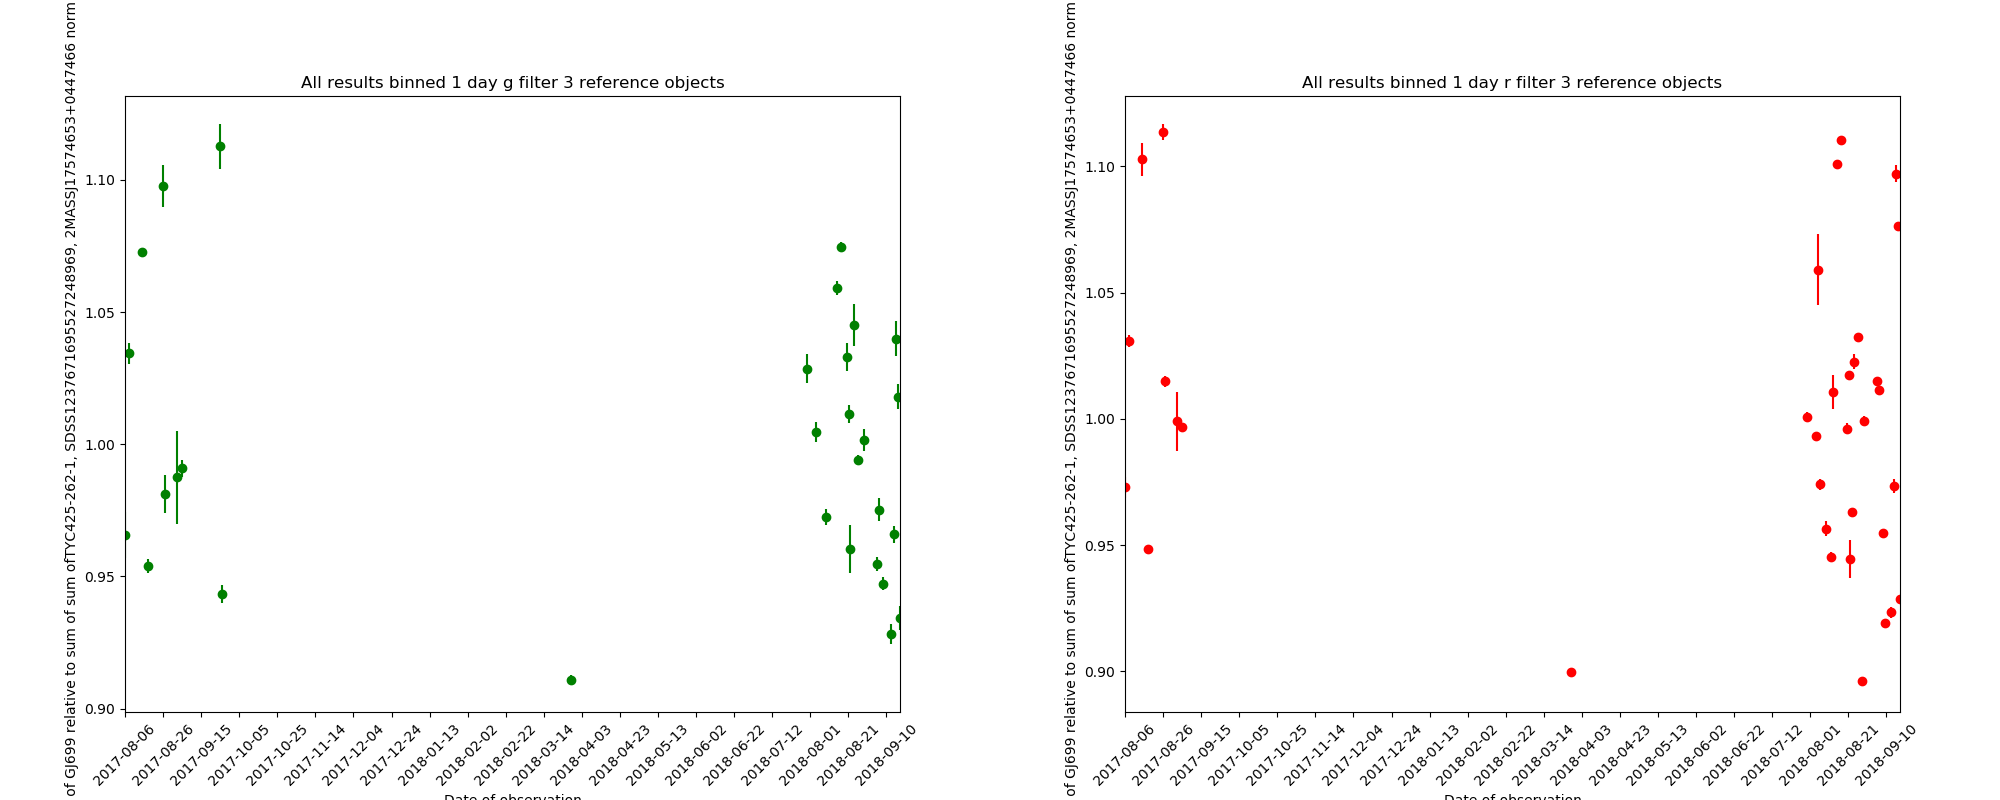
\includegraphics[scale=0.25]{images/allref123bin.png}
\end{center}   
\caption{This shows the ratio of the flux for the target, \bstar, to the 3 main reference objects as per Fig. \ref{fig:allref123} and binned to 1 day.}
  \protect\label{fig:allref123bin}
\end{figure}

\begin{figure}[!htbp]
\begin{center}
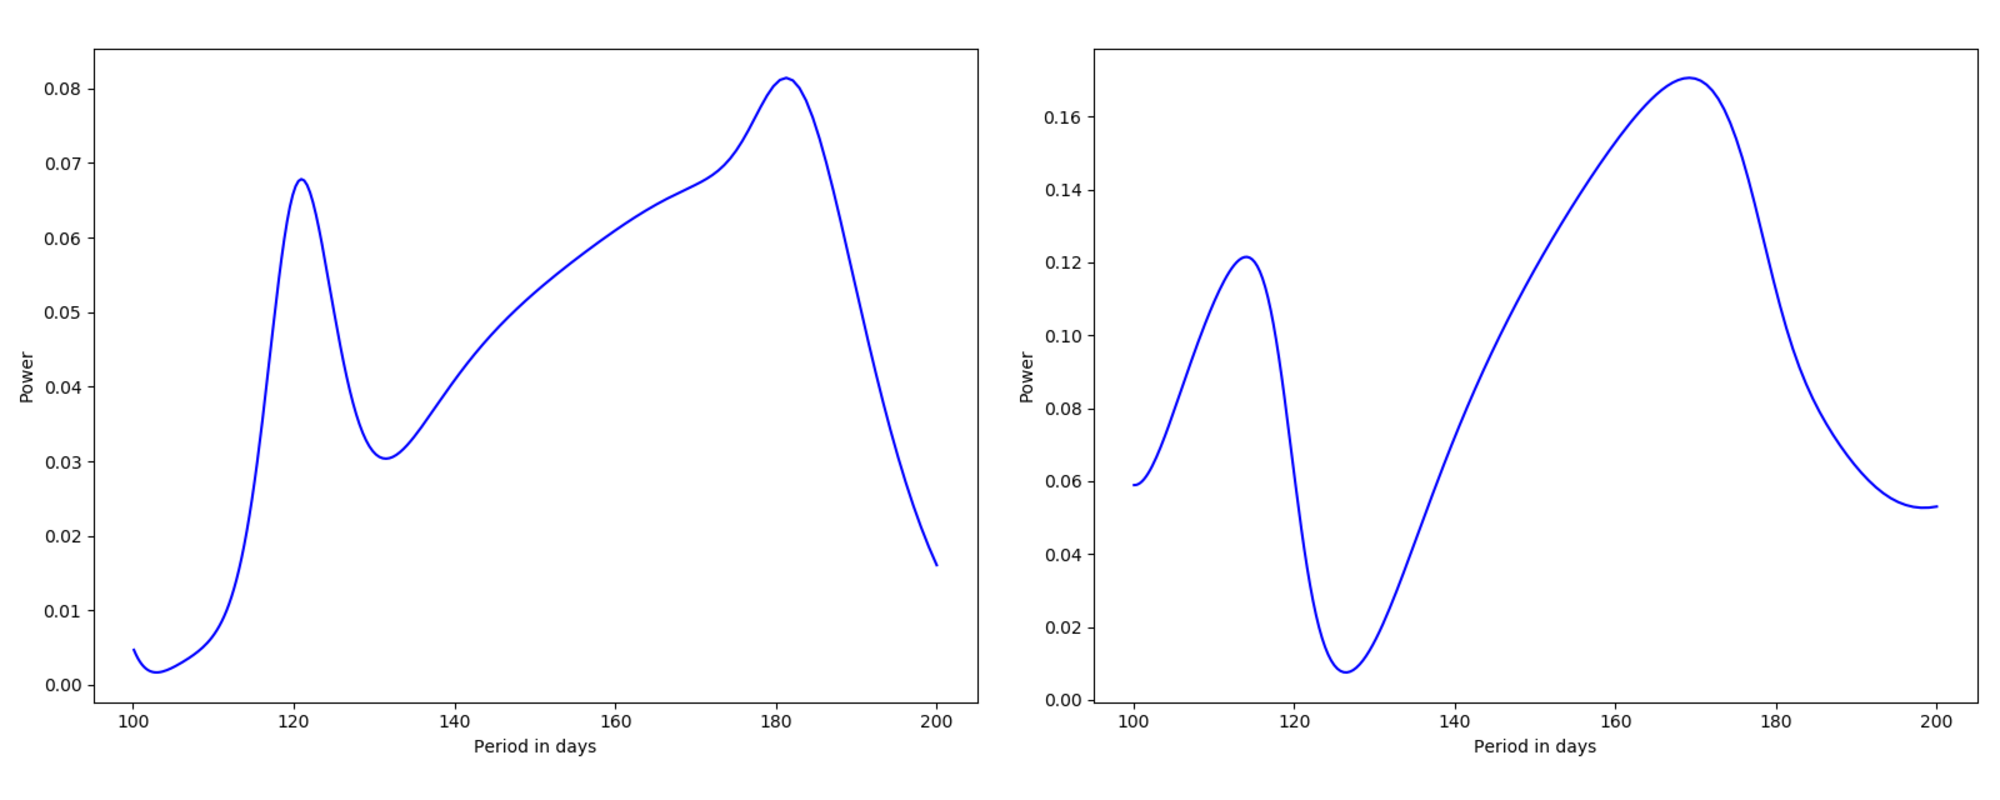
\includegraphics[scale=0.25]{images/ls123both.png}
\end{center}   
\caption{Periodograms obtained from Fig. \ref{fig:allref123}, left panel and Fig. \ref{fig:allref123bin} in right
  panel. Only the \textbf{g} filter was used in this plot, the one from the \textbf{r} filter being almost identical.}
  \protect\label{fig:ls123both}
\end{figure}

\begin{figure}[!htbp]
\begin{center}
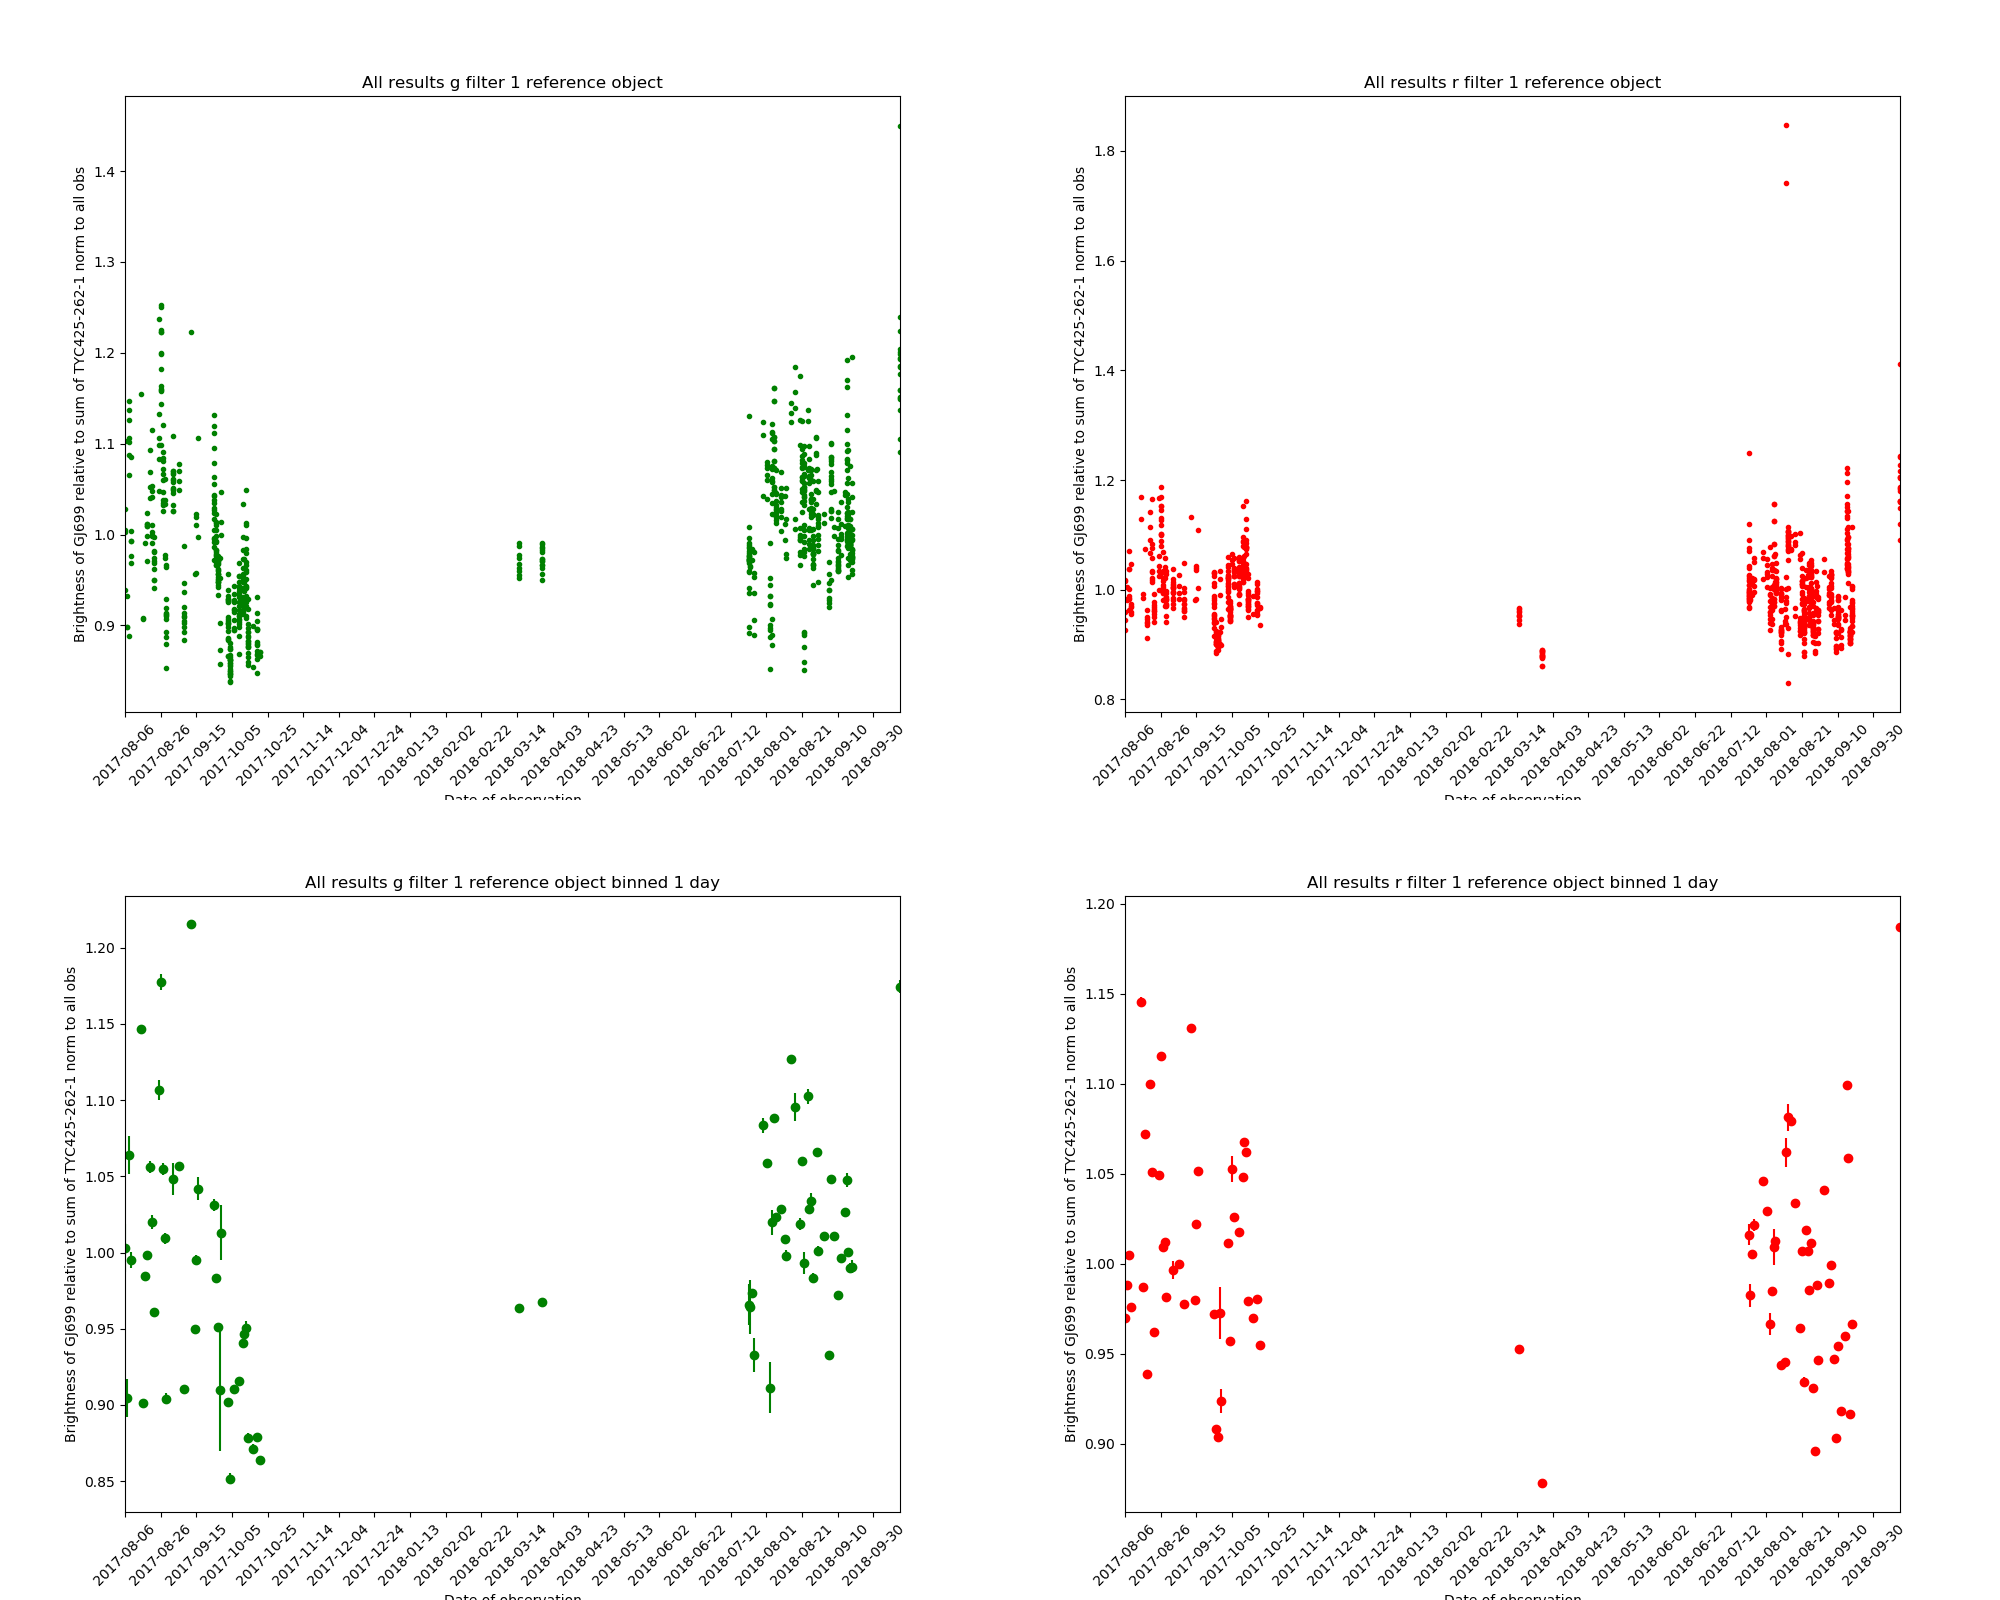
\includegraphics[scale=0.25]{images/allref1.png}
\end{center}   
\caption{This shows the ratio of the flux for the target, \bstar, to the strongest of the reference objects, TYC425-262-1.}
  \protect\label{fig:allref1}
\end{figure}

\begin{figure}[!htbp]
\begin{center}
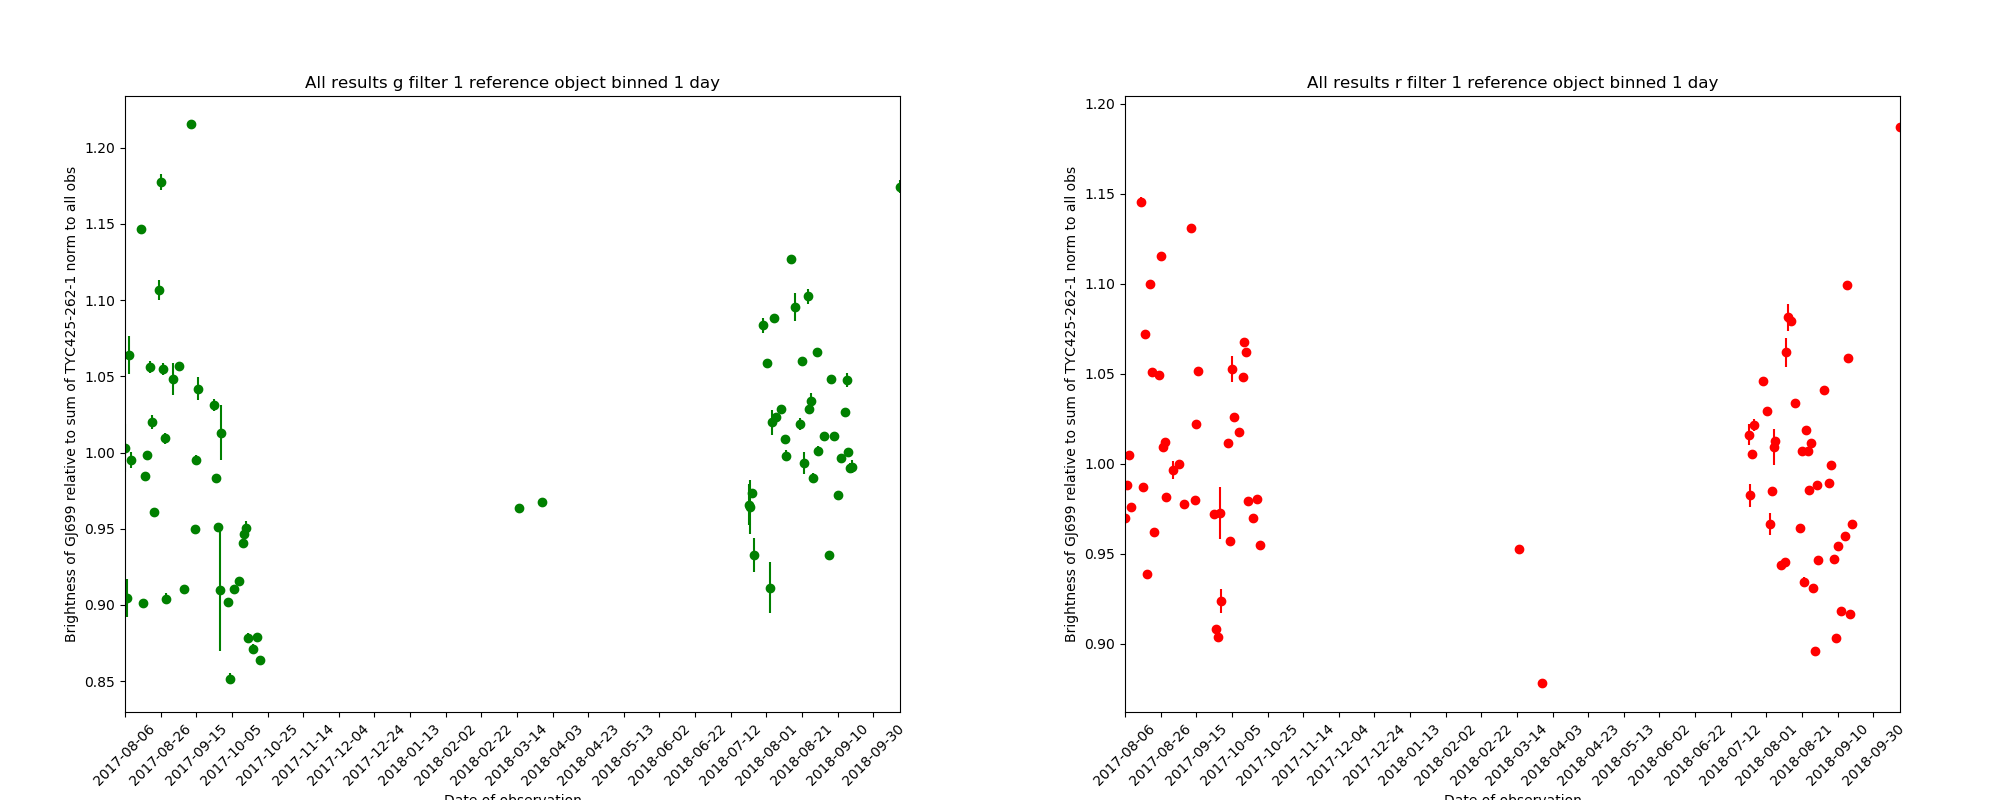
\includegraphics[scale=0.25]{images/allref1bin.png}
\end{center}   
\caption{This shows the ratio of the flux for the target, \bstar, to the strongest of the reference objects,
  TYC425-262-1 per Fig. \ref{fig:allref1} and binned to 1 day.}
  \protect\label{fig:allref1bin}
\end{figure}

\begin{figure}[!htbp]
\begin{center}
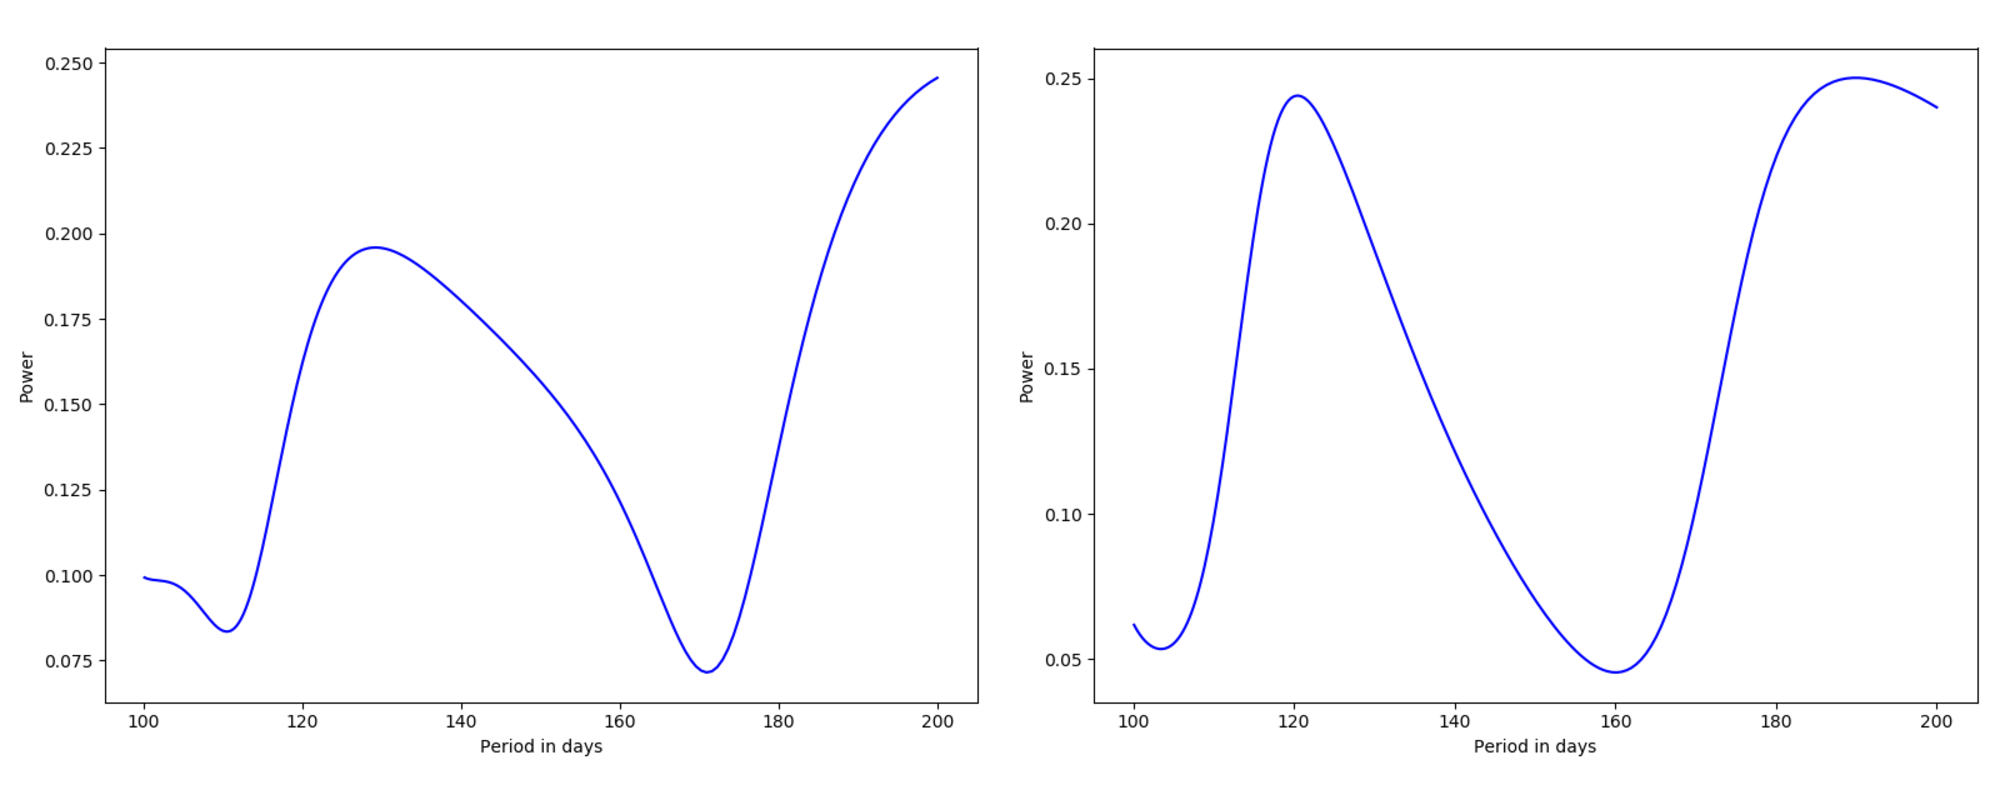
\includegraphics[scale=0.25]{images/ls1both.png}
\end{center}   
\caption{Periodograms obtained from Fig. \ref{fig:allref1}, left panel and Fig. \ref{fig:allref1bin} in right
  panel. Only the \textbf{g} filter was used in this plot, the one from the \textbf{r} filter being almost identical.}
\protect\label{fig:ls1both}
\end{figure}
\clearpage
